% Created 2026-09-20 周日 10:30
% Intended LaTeX compiler: pdflatex
\documentclass[bigger,aspectratio=169]{beamer}
\usepackage[utf8]{inputenc}
\usepackage[T1]{fontenc}
\usepackage{graphicx}
\usepackage{grffile}
\usepackage{longtable}
\usepackage{wrapfig}
\usepackage{rotating}
\usepackage[normalem]{ulem}
\usepackage{amsmath}
\usepackage{textcomp}
\usepackage{amssymb}
\usepackage{capt-of}
\usepackage{hyperref}
\mode<beamer>{\usetheme{AUTheme}}
\setbeamertemplate{caption}[numbered]
\usepackage{color,xpinyin}
\usepackage[normalem]{ulem}
\usepackage{fontspec}
\usepackage{subfigure}
\usepackage{amsmath,array,ulem,qrcode}
\usepackage{xeCJK}
\usepackage{tikz}
\usepackage{bloques}
\usepackage{threeparttable}
\usepackage{mathrsfs}
\setmainfont{Times New Roman}
\usepackage{beamerAppera}
\setCJKmainfont{STSong}
\setsansfont{Times New Roman}
\setlength{\parsep}{0ex}
\setlength{\itemsep}{0ex}
\setlength{\partopsep}{0ex}
\setlength{\topsep}{0ex}
\setlength{\parskip}{0ex}
\setlength{\abovedisplayshortskip}{0pt}
\setlength{\belowdisplayshortskip}{0pt}
\renewcommand{\figurename}{图}
\renewcommand{\tablename}{表}
\hypersetup{colorlinks=true,linkcolor=blue,urlcolor=blue,citecolor=blue}
\usepackage{tcolorbox}
\usepackage{varwidth}
\usetheme{default}
\author{周计明}
\date{2026年 \(\cdot\) 秋}
\title{\fHei 金工实习（冷加工）}
\institute[西工大]{西北工业大学}
\makeatletter
\def\beamer@framenotesbegin{% at beginning of slide
\usebeamercolor[fg]{normal text}
\gdef\beamer@noteitems{}%
\gdef\beamer@notes{}%
}
\makeatother
\graphicspath{{./figures/}}
\DeclareGraphicsExtensions{.pdf,.png,.jpg}
\newtcbox{\mybox}{colback=red!5!white,colframe=red!75!black,varwidth upper,top=0mm,bottom=0mm,left=0mm,right=0mm}
\hypersetup{
 pdfauthor={周计明},
 pdftitle={\fHei 金工实习（冷加工）},
 pdfkeywords={},
 pdfsubject={},
 pdfcreator={Emacs 27.1 (Org mode 9.3)}, 
 pdflang={English}}
\begin{document}

\maketitle
\begin{frame}{Outline}
\tableofcontents
\end{frame}


\section{切削加工概述}
\label{sec:org1c58066}
\begin{frame}[label={sec:org68a2fe5}]{切削加工概述}
\begin{itemize}
\item 使用刀具切除工件毛坯（比如\href{https://www.bilibili.com/video/BV11SbJ6rENs/?share_source=copy_web&vd_source=065b5817f3e3c58ce8d6353b4192b896}{手锤锻件毛坯} ）上多余的金属，使工件达到所需的形状、加工精度和表面质量
\begin{itemize}
\item \alert{机械加工方法} ：车削（\fKai 回转体表面\normalfont）、钻削（\fKai 孔 \normalfont）、镗削（\fKai 大孔、平行孔系 \normalfont）、刨削（\fKai 平面沟槽 \normalfont）、铣削（\fKai 平面沟槽\normalfont）和磨削（\fKai 提高表面精度\normalfont）等。
\item \alert{手工加工方法} ：钳工（\fKai 包括划线、锯削等\normalfont）
\end{itemize}
\end{itemize}

\begin{center}
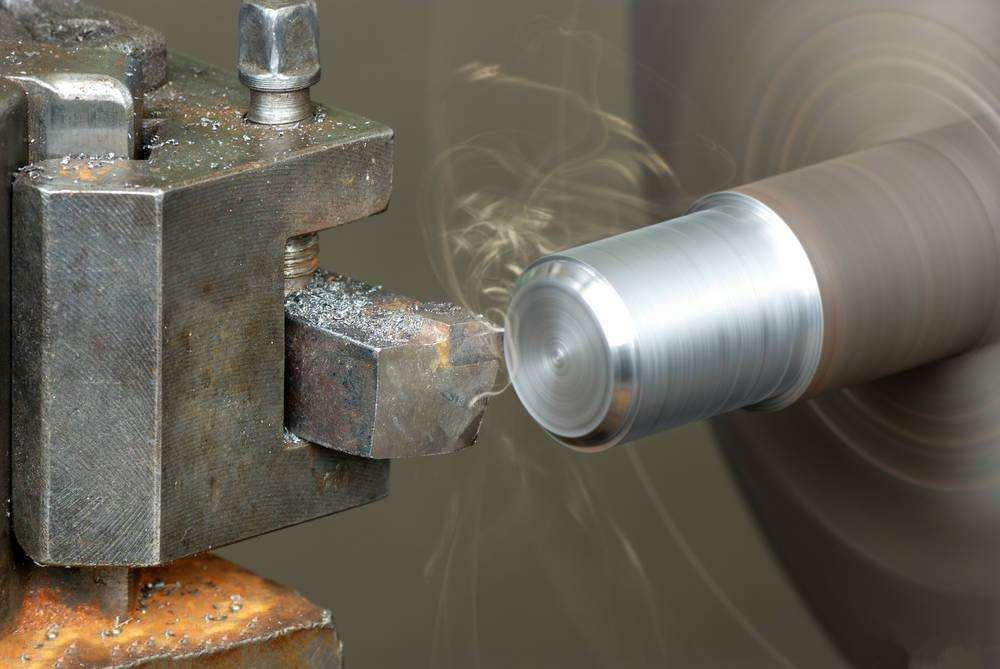
\includegraphics[width=5cm]{./file-20260904233932286.png}
\end{center}
\end{frame}

\section{划线}
\label{sec:org668bc56}
\begin{frame}[label={sec:org0328045}]{划线\footnote{划线只用于指示，最终的精确尺寸必须通过检测来确认}}
在工件的毛坯或已加工表面上，按照图纸要求的尺寸，准确地划出加工界限
\begin{itemize}
\item 指示工件轮廓或孔、槽等特征的位置，合理分配加工余量
\item 指示将工件安装于机器上的位置（\fKai 比如中心孔的位置\normalfont）
\item 检查毛坯外形尺寸是否合乎要求，避免不合格毛坯进入加工环节，造成浪费
\end{itemize}
\end{frame}
\begin{frame}[label={sec:org0b86b24}]{基准 Datum}
\begin{columns}
\begin{column}{0.6\columnwidth}
即参考位置，据此得出所有尺寸从而进行全部测量
\begin{itemize}
\item \alert{点} （\fKai 需要两条基准，且这两条基准通常相互垂直\normalfont）
\item \alert{线} （\fKai 一条边或中心线\normalfont）
\item \alert{面} （\fKai 工件毛坯表面或已加工表面\normalfont）
\end{itemize}

尽量选择已加工面作为基准；加工毛坯时，选择重要的孔或较大的面作为基准
\end{column}

\begin{column}{0.4\columnwidth}
\begin{center}
\includegraphics[page=63, viewport={79.5 405.0 273.5 543.5}, clip,width=5cm]{./WorkshopProcesses.pdf}
\end{center}
\end{column}
\end{columns}
\end{frame}

\begin{frame}[label={sec:org1e70f0d}]{划线工具}
\begin{columns}
\begin{column}{0.4\columnwidth}
\begin{itemize}
\item 平台或平板（\fKai 基准工具\normalfont）
\item 千斤顶（\fKai 夹持工具\normalfont）
\item V型块（夹持工具）
\item 划针（以下为 \fKai 划线工具\normalfont）
\item 划针盘
\item 高度游标尺
\item 划规
\item 单边卡钳
\item 样冲
\end{itemize}
\end{column}
\begin{column}{0.5\columnwidth}
\begin{center}
\includegraphics[page=65, viewport={115.0 60.8 238.6 230.1}, clip,width=5cm]{./WorkshopProcesses.pdf}
\end{center}
\end{column}
\end{columns}
\end{frame}

\begin{frame}[label={sec:orgdf1a786}]{V型块和划针盘}
\begin{center}
\includegraphics[page=64, viewport={253.5 165.5 466.1 316.7}, clip,width=7cm]{./WorkshopProcesses.pdf}
\end{center}
\end{frame}

\begin{frame}[label={sec:orgd359e0b}]{划线染料}
划线前用快干的有色染料喷洒或涂刷于金属表面，使划线清晰可见

\begin{center}
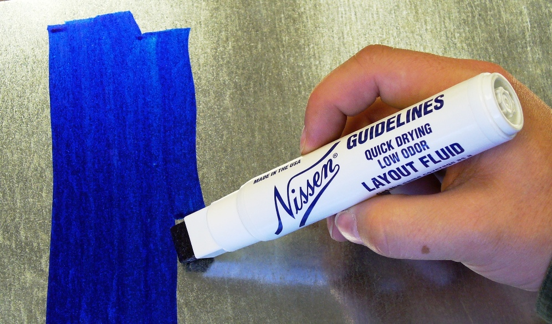
\includegraphics[width=5cm]{./file-20260904164159943.png}
\end{center}
\end{frame}

\section{钳工}
\label{sec:org5052a68}

\begin{frame}[label={sec:org95d9af8}]{钳工}
以手工操作为主，用手工工具去除材料，装配和修理也属于钳工的工作范围。包括：普通钳工、划线钳工、模具钳工、工具钳工、装配钳工、钻工和维修钳工等

\begin{itemize}
\item 锉削
\item 锯切
\item 冷錾
\item 刮削
\item 攻螺纹
\item 套螺纹
\end{itemize}
\end{frame}

\begin{frame}[label={sec:org6a49cb9}]{钳工工作场地和夹具}
\begin{itemize}
\item 钳工工作台
\item 台虎钳
\end{itemize}

\begin{center}
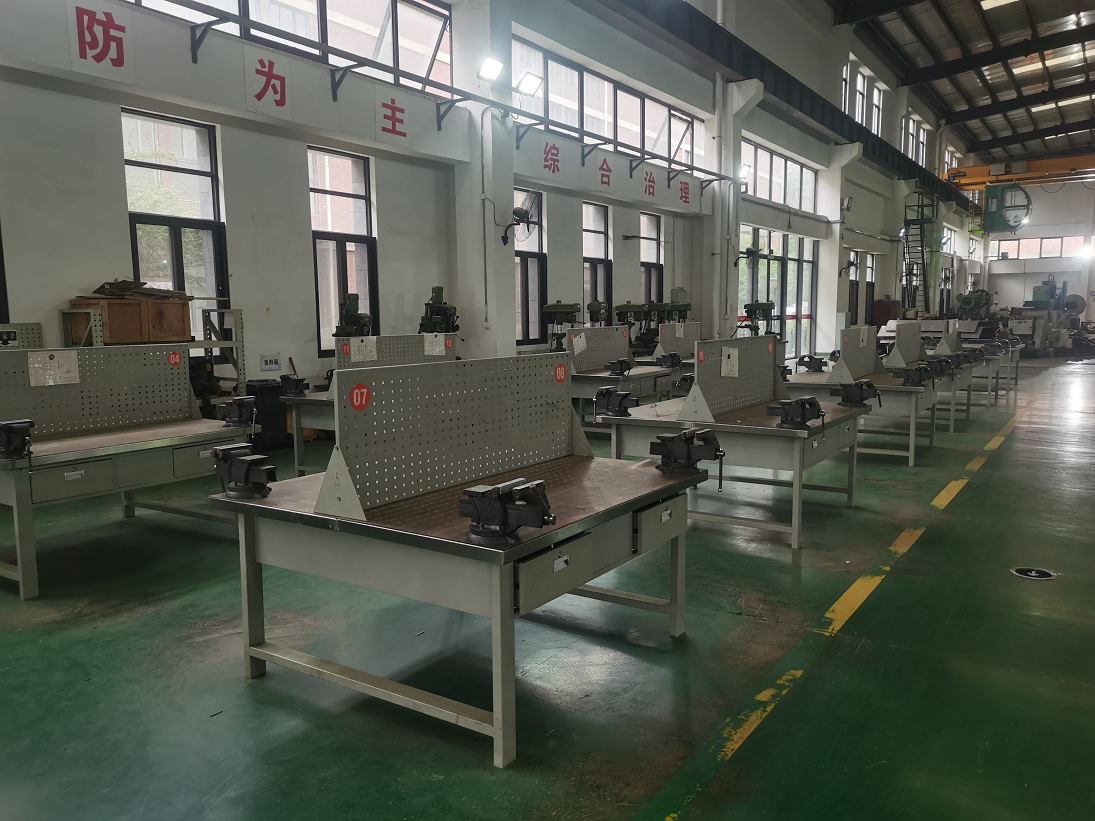
\includegraphics[width=8cm]{./file-20260904234417030.png}
\end{center}
\end{frame}
\begin{frame}[label={sec:org21d40ca}]{锯削}
\begin{itemize}
\item 切断或切槽的重要加工方法
\item 使用手锯进行锯削，手锯由锯弓和锯条组成
\item 锯条根据齿距大小，按每25mm分布的齿数多少分为粗齿（14 \(\sim\) 18）、中齿（22 \(\sim\) 24）和细齿（32）
\begin{itemize}
\item \alert{粗齿} ：铜、铝等软金属，厚件
\item \alert{中齿} ：普通钢、铸铁，中等厚度
\item \alert{细齿} ：硬钢，薄壁件
\end{itemize}
\end{itemize}

\begin{center}
\includegraphics[page=159, viewport={259.5 250.4 467.5 332.4}, clip,width=5cm]{./npupractice.pdf}
\end{center}
\end{frame}

\begin{frame}[label={sec:org255870a}]{锯条的选择}
\begin{itemize}
\item \alert{全硬锯条} ：淬硬高速钢制成，硬度很大，寿命较长，但易断，适合于熟练工
\item \alert{柔性锯条} ：高速钢制成，但仅淬硬锯齿，韧性好，但寿命短，适合于经验不足的人，观看B站视频\href{https://www.bilibili.com/video/BV11SbJ6rENs/?p=2&share_source=copy_web&vd_source=065b5817f3e3c58ce8d6353b4192b896}{钢锯条的铣削加工}
\item \alert{双金属锯条} ：窄的淬硬高速钢锯边和韧性合金锯背经电子束焊而成，寿命长，韧性好
\end{itemize}

\begin{center}
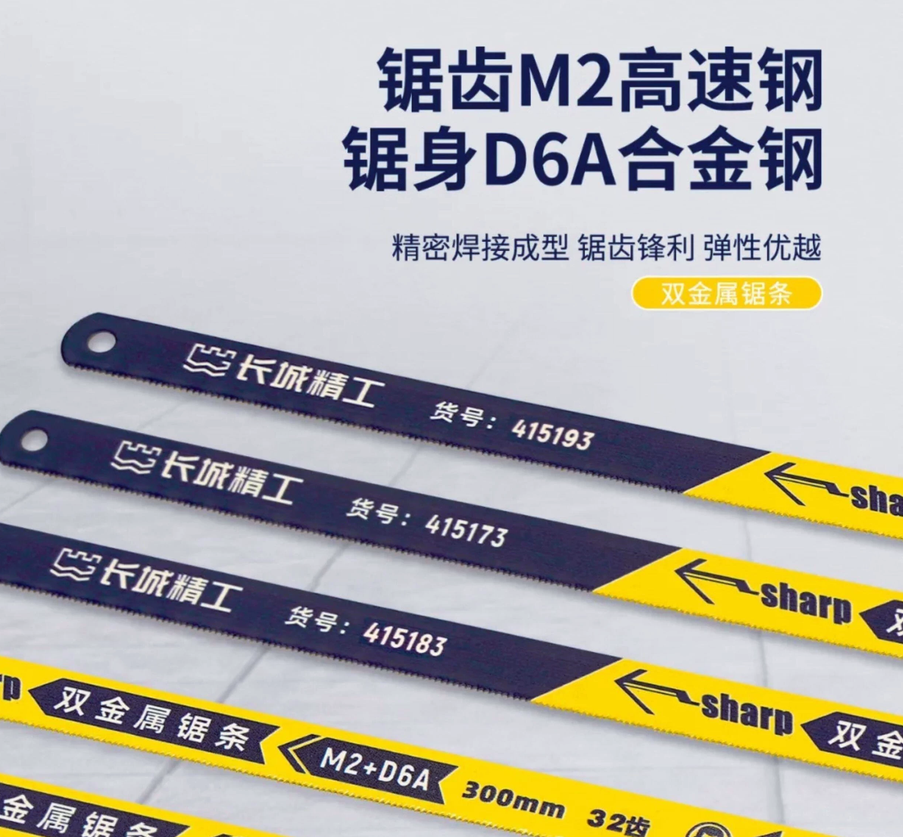
\includegraphics[width=5cm]{./file-20260903175141756.png}
\end{center}
\end{frame}


\begin{frame}[label={sec:orgfaab61c}]{锯削操作}
\begin{itemize}
\item 起锯角度约为 10 \(\sim\) 15\(^\circ\)，角度太大易崩齿，太小不易切入
\item 起锯时往复行程要短，用力要轻，切深2mm后逐渐调至水平正常切削
\end{itemize}

\begin{center}
\includegraphics[page=141, viewport={95.3 538.6 531.5 723.7}, clip,width=8cm]{./metalijxie.pdf}
\end{center}
\end{frame}

\begin{frame}[label={sec:orga1cd5fd}]{锉削}
\begin{itemize}
\item 表面加工，提高精度
\item 锉刀用碳素工具钢制成，经热处理淬硬
\item 齿纹包括单齿纹和双齿纹
\end{itemize}

\begin{center}
\includegraphics[page=143, viewport={49.5 169.0 301.5 303.5}, clip,width=6cm]{./metalijxie.pdf}
\end{center}
\end{frame}

\begin{frame}[label={sec:orgd7dd256}]{锉刀种类}
\begin{itemize}
\item 按用途分：钳工锉、整形锉（什锦锉）、特种锉
\item 按断面形状：平锉、方锉、圆锉、半圆锉和三角锉等
\item 锉刀也分：粗齿（4 \(\sim\) 12）、中齿（13 \(\sim\) 23）、细齿（30 \(\sim\) 40）以及油光锉（50 \(\sim\) 62），按每10mm长度内锉面上的齿数
\end{itemize}

\begin{center}
\includegraphics[page=50, viewport={252.5 51.0 470.5 127.5}, clip,width=7cm]{./WorkshopProcesses.pdf}
\end{center}
\end{frame}

\begin{frame}[label={sec:org1855d81}]{平面锉削操作}
\begin{itemize}
\item 锉刀向运动时进行切削，锉刀退回时不抬离工件，有利于去除锉齿上的锉屑，但不施加压力
\end{itemize}

\begin{center}
\includegraphics[page=145, viewport={96.0 175.5 532.5 360.0}, clip,width=10cm]{./metalijxie.pdf}
\end{center}
\end{frame}

\begin{frame}[label={sec:org1b2d1d2}]{曲面锉削操作}
图示依次是：滚锉、横锉、锉削内圆弧面、锉削球面
\begin{center}
\includegraphics[page=146, viewport={101.5 156.5 485.0 418.5}, clip,width=9cm]{./metalijxie.pdf}
\end{center}
\end{frame}

\section{切削刀具}
\label{sec:orga5bba79}

\begin{frame}[label={sec:org74d1db2}]{切削刀具}
\begin{itemize}
\item 切削刀具的材料：红硬度、耐磨性和韧性
\begin{itemize}
\item 高速钢、硬质合金（\fKai 碳化钨等硬质颗粒与黏结金属组成粉末经粉末冶金制成\normalfont）
\end{itemize}
\item 切削刀具的几何角度（\fKai 前角和后角\normalfont）
\item 车刀结构（\fKai 三面两刃一尖\normalfont）
\item 切削速度（\fKai 刀具或工件的表面速度\normalfont）
\end{itemize}
\end{frame}

\begin{frame}[label={sec:orgdb6753d}]{切削速度}
\begin{itemize}
\item 切削刀具与工件之间的相对速度，单位m/min
\begin{itemize}
\item 车削是工件的表面速度，铣削钻削时是刀具的表面速度
\end{itemize}
\end{itemize}

\[cutting\ speed\ S = \frac{\pi dN}{1000} \rm m/min \]

\begin{center}
\includegraphics[page=128, viewport={294.0 213.0 422.0 289.0}, clip,width=6cm]{./WorkshopProcesses.pdf}
\end{center}
\end{frame}

\begin{frame}[label={sec:org28af4cb}]{刀具的后角 Clearance 和前角 rake}
\begin{figure}[htbp]
\centering
\includegraphics[page=122, viewport={256.5 527.0 461.0 605.5}, clip,width=6cm]{./WorkshopProcesses.pdf}
\caption{刀具后角}
\end{figure}

\begin{figure}[htbp]
\centering
\includegraphics[page=123, viewport={79.5 379.0 276.0 461.0}, clip,width=6cm]{./WorkshopProcesses.pdf}
\caption{刀具前角}
\end{figure}
\end{frame}

\begin{frame}[label={sec:org1fd0c8d}]{不同刀具的前角和后角}
\begin{center}
\includegraphics[page=123, viewport={147.5 38.5 428.5 292.5}, clip,width=8cm]{./WorkshopProcesses.pdf}
\end{center}
\end{frame}

\begin{frame}[label={sec:orgfee1155}]{车刀刀具角度}
\begin{itemize}
\item 三个辅助平面：基面、切削平面、主剖面
\item 三面两刃一尖
\begin{itemize}
\item 前面、主后面、副后面
\item 主切削刃、副切削刃
\item 刀尖
\end{itemize}
\end{itemize}
\begin{center}
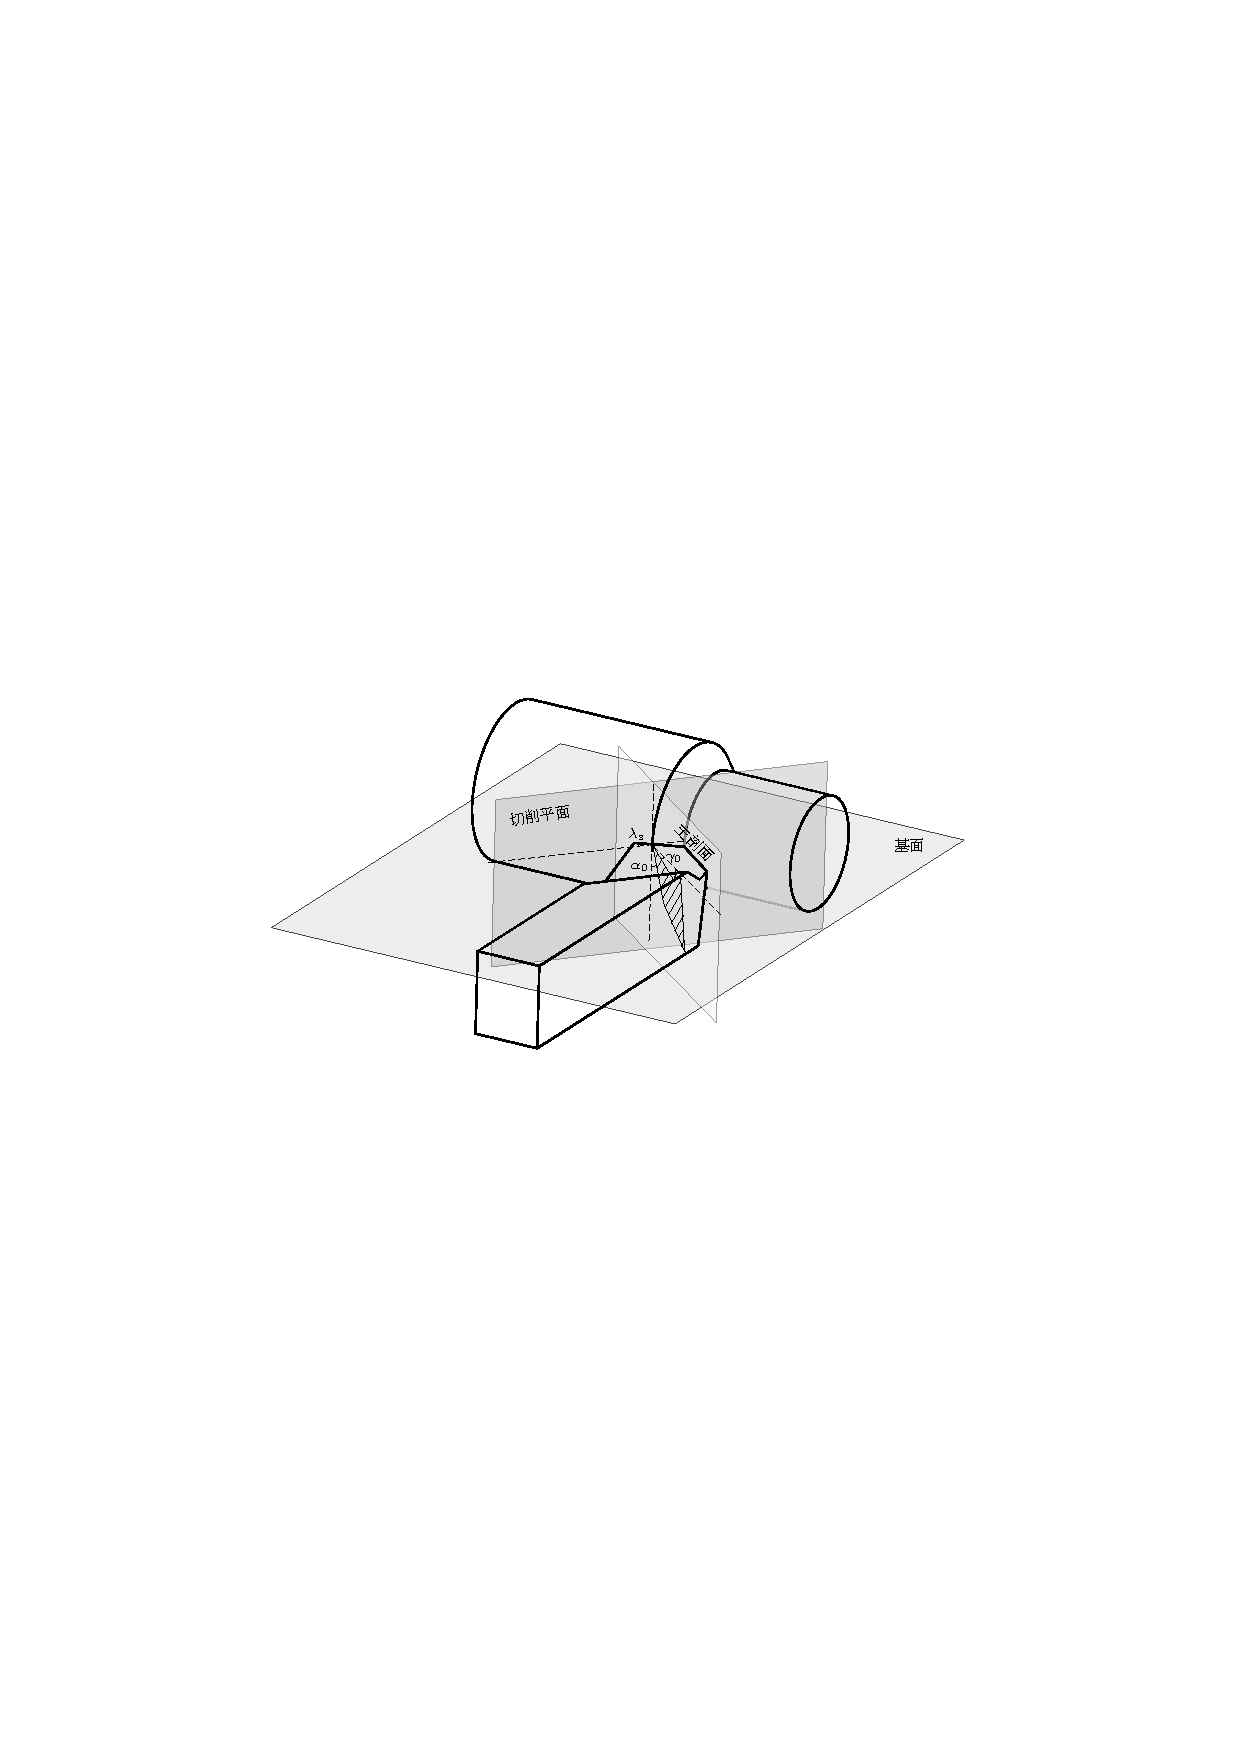
\includegraphics[width=10cm]{./fig0406.pdf}
\end{center}
\end{frame}

\section{车削}
\label{sec:org41048e8}

\begin{frame}[label={sec:orge67c587}]{车削工作范围}
\begin{itemize}
\item 回转体表面（\fKai 包括内表面和外表面\normalfont）的主要加工方法
\item 阶梯轴
\item 车螺纹
\item 切断
\end{itemize}

\begin{center}
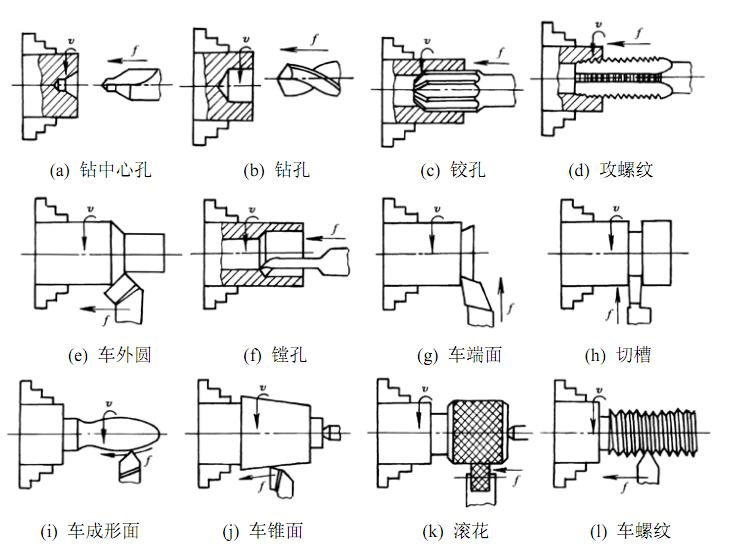
\includegraphics[width=6cm]{./file-20260904234944100.png}
\end{center}
\end{frame}

\begin{frame}[label={sec:orgc70ad08}]{车床结构}
\begin{itemize}
\item 主轴箱实现变速，通过带传动、齿轮传动将电机转动传送到主轴，主轴的调速范围在40 \(\sim\) 2500 r/min之间
\end{itemize}
\begin{center}
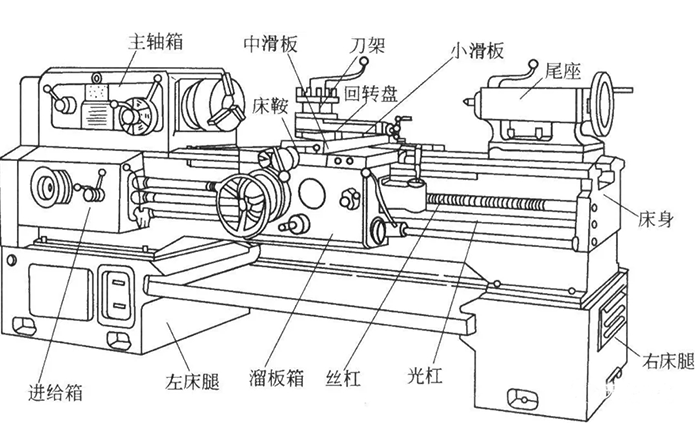
\includegraphics[width=8cm]{./file-20260904092320073.png}
\end{center}
\end{frame}

\begin{frame}[label={sec:orgd4b5e30}]{溜板箱和刀架}
\begin{center}
\includegraphics[page=46, viewport={117.3 472.5 464.6 748.1}, clip,width=8cm]{./metalijxie.pdf}
\end{center}

\begin{itemize}
\item 溜板箱与床鞍相连，是车床进给运动的操纵箱，通过光杠或丝杠驱动其运动，进而带动刀架进行直线运动
\item 刀架用来安装刀具
\end{itemize}
\end{frame}

\begin{frame}[label={sec:orgd421481}]{零件装夹}
\begin{itemize}
\item \alert{三爪卡盘} ：三个卡爪同时移动，自定心，装夹小型轴类、盘套类零件
\item \alert{四爪卡盘} ：四个卡爪独立移动，夹紧力大，安装调整困难，不规则的较大零件
\item \alert{夹头} 安装轴类零件
\item \alert{花盘} ：大直径铸铁圆盘，有时配合弯板装夹工件
\item \alert{顶尖} ：装夹轴类零件（\fKai 需要配合拔盘和鸡心夹头\normalfont）
\item \alert{跟刀架和中心架} ：防止细长轴变形
\end{itemize}
\end{frame}

\begin{frame}[label={sec:org52fae7d}]{前后顶尖装夹工件}
\begin{itemize}
\item 双顶尖装夹工件，通过两端面锥面定位，定位精度高
\end{itemize}
\begin{columns}
\begin{column}{0.6\columnwidth}
\begin{center}
\includegraphics[page=55, viewport={347.2 535.5 561.4 739.4}, clip,width=6cm]{./metalijxie.pdf}
\end{center}
\end{column}
\begin{column}{0.4\columnwidth}
\begin{center}
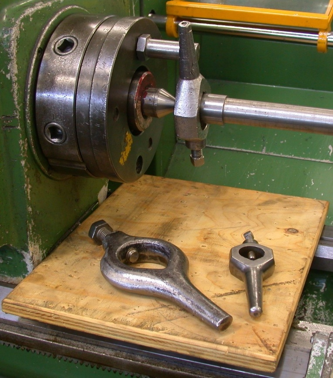
\includegraphics[width=5cm]{./file-20260904165004333.png}
\end{center}
\end{column}
\end{columns}
\end{frame}

\begin{frame}[label={sec:orga1b15d6}]{跟刀架和中心架}
\begin{itemize}
\item 跟刀架固定在床鞍上跟随刀架一起移动，适合光轴加工
\item 中心架固定在床身上，如可用于车削长轴端面或镗内孔时
\end{itemize}

\begin{center}
\includegraphics[page=56, viewport={40.2 103.2 500.8 254.4}, clip,width=11cm]{./metalijxie.pdf}
\end{center}
\end{frame}

\begin{frame}[label={sec:org29e6983}]{花盘装夹不规则零件}
\begin{itemize}
\item 盘面上许多长槽用来穿入压紧螺栓，花盘端面与其轴线垂直
\item 为减小质量偏心引起的振动，还需要加平衡块
\end{itemize}

\begin{center}
\includegraphics[page=58, viewport={312.6 533.1 548.8 708.7}, clip,width=8cm]{./metalijxie.pdf}
\end{center}
\end{frame}

\section{铣削}
\label{sec:org8199c4d}

\begin{frame}[label={sec:orga745835}]{铣削}
\begin{itemize}
\item 平面、沟槽、成形面的主要加工方法
\item 设备：卧式铣床和立式铣床
\item 夹具：旋转工作台和分度头
\end{itemize}

\begin{center}
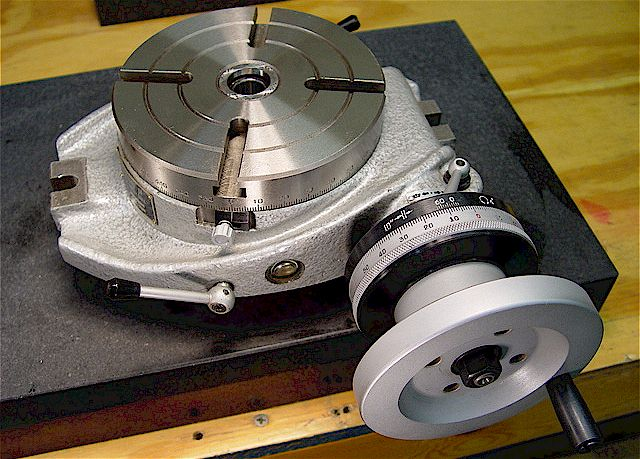
\includegraphics[width=5cm]{./file-20260904165131867.png}
\end{center}
\end{frame}

\begin{frame}[label={sec:org9107c75}]{卧式铣床和立式铣床}
\begin{columns}[b]
\begin{column}{0.5\columnwidth}
\begin{figure}[htbp]
\centering
\includegraphics[page=117, viewport={235.5 171.4 487.5 412.9}, clip,width=5cm]{./npupractice.pdf}
\caption{卧式铣床}
\end{figure}
\end{column}

\begin{column}{0.5\columnwidth}
\begin{figure}[htbp]
\centering
\includegraphics[page=118, viewport={177.5 123.9 424.0 402.9}, clip,width=5cm]{./npupractice.pdf}
\caption{立式铣床}
\end{figure}
\end{column}
\end{columns}
\end{frame}


\begin{frame}[label={sec:orga21e4aa}]{铣刀及铣削工作}
观看B站视频\href{https://www.bilibili.com/video/BV1rZbJ6KErG/?share_source=copy_web&vd_source=065b5817f3e3c58ce8d6353b4192b896}{铣刀的铣削加工}

\begin{columns}
\begin{column}{0.5\columnwidth}
\begin{center}
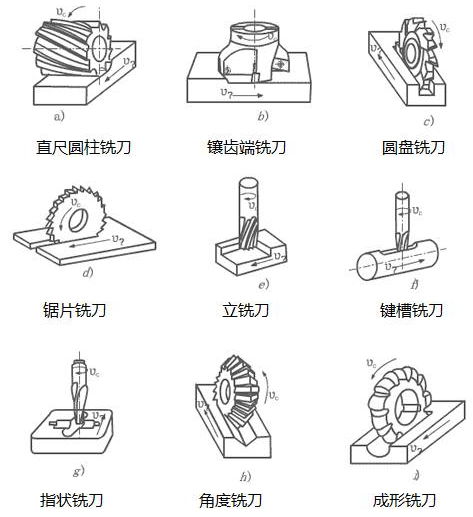
\includegraphics[height=5cm]{./file-20260904235329720.png}
\end{center}
\end{column}
\begin{column}{0.5\columnwidth}
\begin{center}
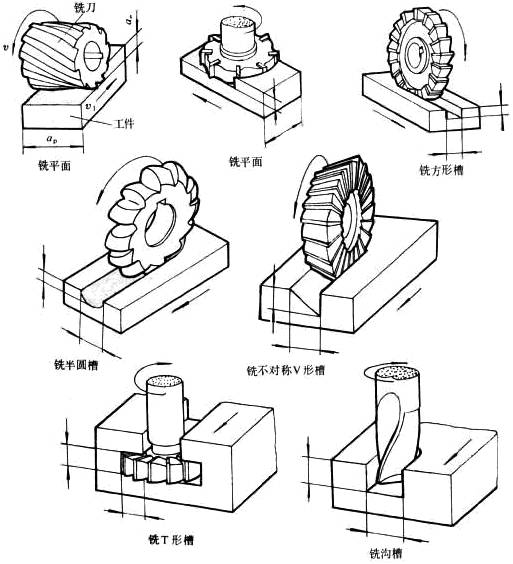
\includegraphics[height=5cm]{./file-20260904235341984.png}
\end{center}
\end{column}
\end{columns}
\end{frame}
\begin{frame}[label={sec:org5c6d56c}]{分度头}
\begin{columns}[b]
\begin{column}{0.6\columnwidth}
\begin{center}
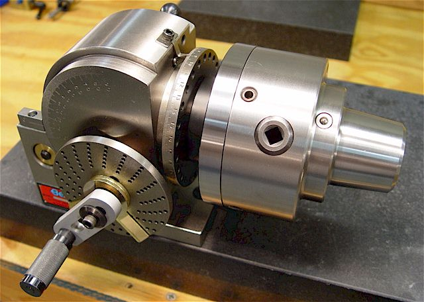
\includegraphics[height=5cm]{./file-20260904165150970.png}
\end{center}
\end{column}

\begin{column}{0.4\columnwidth}
\begin{center}
\includegraphics[page=87, viewport={303.1 529.2 564.6 770.9}, clip,width=5cm]{./metalijxie.pdf}
\end{center}
\end{column}
\end{columns}
\end{frame}

\begin{frame}[label={sec:orgcfaca57}]{铣削方式--顺铣与逆铣}
\begin{itemize}
\item \alert{顺铣} ：铣刀与工件接触处的旋转方向和工件的进给方向相同
\item \alert{逆铣} ：铣刀切削刃的运动方向和工件的进给方向相反
\end{itemize}

\begin{center}
\includegraphics[page=91, viewport={292.1 514.2 553.5 687.5}, clip,width=7cm]{./metalijxie.pdf}
\end{center}
\end{frame}

\section{工程材料及热处理}
\label{sec:orgd563823}
\begin{frame}[label={sec:orgedb3f1d}]{工程材料及其分类}
\begin{itemize}
\item 各种工程领域中应用的材料
\end{itemize}

\begin{center}
\includegraphics[page=18, viewport={113.0 95.9 483.0 226.9}, clip,width=10cm]{./metaljixiehot.pdf}
\end{center}
\end{frame}

\begin{frame}[label={sec:orgac882a4}]{工程材料的性能}
\begin{itemize}
\item 物理性能
\begin{itemize}
\item 线膨胀系数、比热容、密度、熔点、热导率、电阻率
\end{itemize}
\item 力学性能
\begin{itemize}
\item 硬度（\fKai 布氏硬度、洛氏硬度\normalfont ）、脆性、强度（\fKai 屈服强度和抗拉强度\normalfont ）、延性 ductility（\fKai 关注拉力作用下的变形能力\normalfont ）、可锻性 malleability（\fKai 关注压应力作用下的变形能力\normalfont ）、弹性、韧性toughness（\fKai 断裂前吸收变形能量的能力\normalfont）
\end{itemize}
\item 工艺性能
\begin{itemize}
\item 铸造性能、锻压性能、焊接性能、切削加工性能
\end{itemize}
\end{itemize}
\end{frame}

\begin{frame}[label={sec:org99693f3}]{典型材料性能对比}
\begin{center}
\begin{tabular}{lrrr}
\hline
类型 & 密度/(kg\(\cdot\) m\textsuperscript{-3}) & 抗拉强度/(MPa) & 熔点/(\(^\circ \rm C\))\\
\hline
低碳钢 & 7800 & 505 & 1495\\
灰铸铁 & \(\sim\) 7200 & 150\(\sim\) 400 & 1100\\
铜 & 8900 & 216 & 1083\\
铝 & 2700 & 80 & 660\\
铝合金 & 2790 & 250 & 600\\
\hline
\end{tabular}
\end{center}
\end{frame}

\begin{frame}[label={sec:orge29585b}]{铁碳合金（钢铁）}
\begin{itemize}
\item 碳的质量分数低于2\%是钢，高于2\%是铁
\item \alert{碳素钢} ：主要成分是铁和碳，包括\uwave{碳素结构钢}和\uwave{碳素工具钢}
\item \alert{合金钢} ：除铁和碳外，还包括一种或几种合金元素，包括\uwave{合金结构钢}和\uwave{合金工具钢}
\item \alert{铸铁} ：碳的质量分数在2.5\%\(\sim\) 4.0\%之间，并含有硅、锰、硫、磷等杂质元素。包括灰铸铁、球墨铸铁和可锻铸铁等（\fKai 石墨存在形态不同\normalfont ）
\end{itemize}

\begin{center}
\includegraphics[page=233, viewport={292.0 227.0 505.5 321.0}, clip,width=6cm]{./WorkshopProcesses.pdf}
\end{center}
\end{frame}

\begin{frame}[label={sec:orgbe94443}]{钢铁材料的牌号}
\begin{itemize}
\item \alert{碳素钢}
\begin{itemize}
\item 普通碳素结构钢 \uwave{Q + 屈服点数值（MPa）}，Q195, Q235，铆钉、螺钉、螺母等
\item 优质碳素结构钢 \uwave{两位数字}表示含碳量的万分数，08、45、65，轴、连杆、齿轮等
\item 碳素工具钢 \uwave{T + 含碳量的千分数} T8、T10、T12等，手钳、锤子、锯条、锉刀等
\end{itemize}
\item \alert{合金钢} 
\begin{itemize}
\item 合金结构钢 \uwave{两位数字+元素符号+数字}，40Cr
\item 合金工具钢 \uwave{一位数字+元素符号+数字}，9SiC，W18Cr4V
\end{itemize}
\item \alert{灰铸铁} \uwave{HT+最低抗拉强度值}，HT150、HT200
\end{itemize}
\end{frame}

\begin{frame}[label={sec:org09160fd}]{热处理}
\begin{itemize}
\item 对固态金属进行一次或多次地加热和冷却以获得所需力学性能的过程
\item 冷却速度对钢的组织影响很大，依据冷却速度的不同，热处理分为： \alert{退火、正火、淬火和回火}
\end{itemize}
\begin{center}
\includegraphics[page=231, viewport={74.5 483.0 280.5 623.5}, clip,width=8cm]{./WorkshopProcesses.pdf}
\end{center}
\end{frame}

\begin{frame}[label={sec:org7ccdc86}]{热处理的加热温度范围}
\begin{itemize}
\item \alert{退火} （\fKai 随炉冷却\normalfont ）、 \alert{正火} （\fKai 出炉空气中冷却\normalfont ）、 \alert{淬火} （\fKai 水冷或油冷\normalfont ）和 \alert{回火} （\fKai 高温、中温、低温回火\normalfont ）
\end{itemize}
\begin{columns}
\begin{column}{0.4\columnwidth}
\begin{itemize}
\item 退火：使钢软化，增加延性，降低强度
\item 正火：强度高于退火，但延性更小
\item 淬火：强化金属，提高硬度
\item 回火：降低硬度，提高韧性
\end{itemize}
\end{column}
\begin{column}{0.6\columnwidth}
\begin{center}
\includegraphics[page=231, viewport={306.0 226.5 492.5 358.5}, clip,width=7cm]{./WorkshopProcesses.pdf}
\end{center}
\end{column}
\end{columns}
\end{frame}

\begin{frame}[label={sec:org827a75f}]{回火温度与硬度的关系}
\begin{itemize}
\item 淬火后进行回火，降低硬度和脆性，恢复韧性
\item 淬火温度越高，钢的韧性越好
\end{itemize}
\begin{center}
\includegraphics[page=233, viewport={69.5 544.0 278.5 662.0}, clip,width=9cm]{./WorkshopProcesses.pdf}
\end{center}
\end{frame}

\section{铸造}
\label{sec:orgd18f9bd}

\begin{frame}[label={sec:org4b3f6f6}]{砂型铸造}
\begin{columns}
\begin{column}{0.5\columnwidth}
\begin{itemize}
\item 数量多少均可
\item 复杂形状、特别是复杂内腔的零件
\item 模具成本低
\item 黑色、有色金属均可
\item 生产效率低
\item 不能生成薄壁件
\item 表面质量差
\end{itemize}
\end{column}

\begin{column}{0.5\columnwidth}
\begin{center}
\includegraphics[page=269, viewport={319.5 52.5 468.5 218.5}, clip,width=6cm]{./WorkshopProcesses.pdf}
\end{center}
\end{column}
\end{columns}
\end{frame}

\begin{frame}[label={sec:org4946615}]{砂型铸造的基本步骤}
\begin{itemize}
\item 配制型（芯）砂、模样准备 \(\rightarrow\) 造型 \(\rightarrow\) 浇注 \(\rightarrow\) 冷却凝固  \(\rightarrow\) 落砂清理 \(\rightarrow\) 检验 \(\rightarrow\) 合格铸件
\end{itemize}
\begin{center}
\includegraphics[page=270, viewport={112.0 519.0 378.5 659.0}, clip,width=10cm]{./WorkshopProcesses.pdf}
\end{center}
\end{frame}

\begin{frame}[label={sec:org5f88bc3}]{模样准备}
\begin{itemize}
\item 模样、底板、砂箱按一定空间位置放置好，填入型砂并舂紧
\item 用手将模样周围的型砂压紧（如图）
\item 填砂时分批加入，每一次填砂，均应舂紧才能再次加砂
\item 舂砂时用力适中，力过大，砂型过紧，不利于气体逸出，过小易塌箱
\end{itemize}
\begin{center}
\includegraphics[page=34, viewport={335.0 92.4 539.5 208.4}, clip,width=6cm]{./metaljixiehot.pdf}
\end{center}
\end{frame}

\begin{frame}[label={sec:org167d747}]{型砂}
\begin{itemize}
\item 具有渗透性（\fKai 多孔性\normalfont ），允许气体和蒸汽逸出
\item 足够强度承受大量熔融金属
\item 耐高温，且颗粒大小适中
\item 型砂的粘合方式
\begin{itemize}
\item \alert{湿砂型} ：由粘土粘结，需仔细控制湿度水平
\item \alert{干砂型} ：前期制作方法与粘土粘结一样，模具做好后加热到100 \(^\circ\)C以上干燥去除水分
\item \alert{CO\(_2\)水玻璃砂型} ：以硅酸钠代替火粘土进行粘结，模具做好后通CO\(_2\)气体进行固化，铸后易破碎
\item \alert{树脂砂型} ：使用有机或无机粘结剂粘合，尺寸控制良好，表面粗糙度低
\end{itemize}
\end{itemize}
\end{frame}
\begin{frame}[label={sec:orgf3d0f07}]{型芯}
\begin{columns}
\begin{column}{0.6\columnwidth}
\begin{itemize}
\item 用于铸造具有空腔的铸件，要足够坚固，有时需要用钢丝来强化强度（\fKai 芯骨 \normalfont）
\item 利用型芯盒单独制作，以模型上的型芯座为底座，支撑定位于模具中
\end{itemize}
\end{column}
\begin{column}{0.4\columnwidth}
\begin{center}
\includegraphics[page=44, viewport={423.7 116.1 544.3 296.4}, clip,width=4cm]{./metaljixiehot.pdf}
\end{center}
\end{column}
\end{columns}
\end{frame}

\begin{frame}[label={sec:orgce087ce}]{真空铸造（V法铸造）}
\begin{itemize}
\item 砂型铸造的变体，使用不含水或粘结剂的干砂造型，模具型腔通过真空保持一定的形状
\item 无需拔模角，最小壁厚可达2.3mm
\item 尺寸精度高，表面粗糙度低，细节重现良好
\end{itemize}
\begin{columns}
\begin{column}{0.6\columnwidth}
\begin{center}
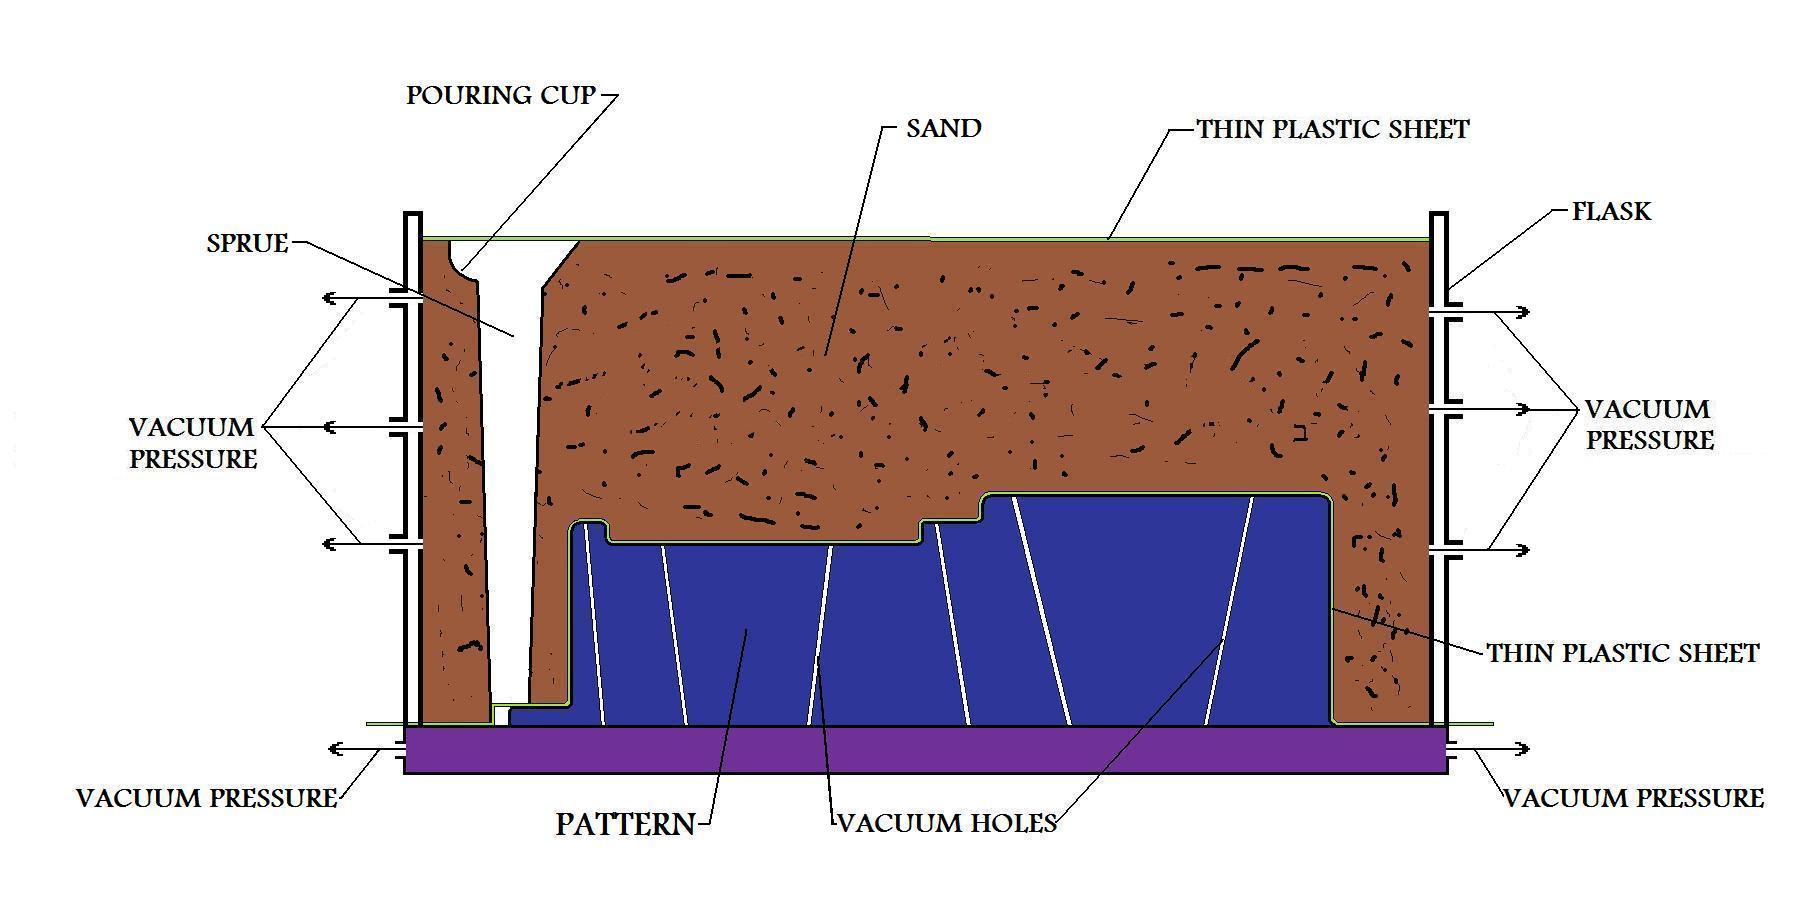
\includegraphics[width=6cm]{./Vacuum_mold4.jpg}
\end{center}
\end{column}

\begin{column}{0.4\columnwidth}
\begin{center}
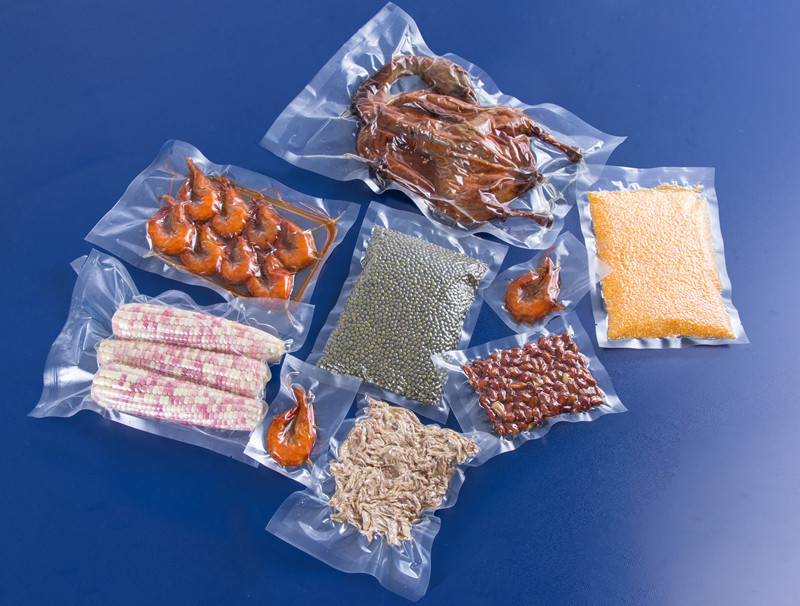
\includegraphics[width=4cm]{./10711812913_673781158.jpg}
\end{center}
\end{column}
\end{columns}
\end{frame}

\begin{frame}[label={sec:org84af4da}]{熔模铸造（失蜡铸造）}
制作蜡模 \(\rightarrow\) 涂挂耐火材料 \(\rightarrow\) 干燥结壳（熔模壳） \(\rightarrow\) 加热焙烧熔模，蜡模流出，形成浇注型腔 \(\rightarrow\) 浇注、凝固 \(\rightarrow\) 清理模壳，获得铸件
\begin{columns}
\begin{column}{0.3\columnwidth}
\begin{center}
\includegraphics[page=291, viewport={72.0 516.0 285.0 654.5}, clip,width=3cm]{./WorkshopProcesses.pdf}
\end{center}
\end{column}
\begin{column}{0.3\columnwidth}
\begin{center}
\includegraphics[page=291, viewport={295.5 459.0 506.5 656.5}, clip,width=3cm]{./WorkshopProcesses.pdf}
\end{center}
\end{column}
\begin{column}{0.3\columnwidth}
\begin{center}
\includegraphics[page=291, viewport={295.0 64.0 504.0 239.0}, clip,width=3cm]{./WorkshopProcesses.pdf}
\end{center} 
\end{column}
\end{columns}
\begin{columns}
\begin{column}{0.3\columnwidth}
\begin{center}
\includegraphics[page=292, viewport={28.0 322.5 241.5 495.0}, clip,width=3cm]{./WorkshopProcesses.pdf}
\end{center}
\end{column}
\begin{column}{0.3\columnwidth}
\begin{center}
\includegraphics[page=292, viewport={253.5 444.5 463.0 655.5}, clip,width=3cm]{./WorkshopProcesses.pdf}
\end{center}
\end{column}
\begin{column}{0.3\columnwidth}
\begin{center}
\includegraphics[page=292, viewport={254.0 258.5 464.0 402.0}, clip,width=3cm]{./WorkshopProcesses.pdf}
\end{center}
\end{column}
\end{columns}
\end{frame}

\begin{frame}[label={sec:org8536bc6}]{改进的熔模铸造工艺}
\begin{columns}
\begin{column}{0.6\columnwidth}
\begin{itemize}
\item 反重力低压空气熔体（Counter gravity low pressure air melt, CLA）铸造工艺，浇注前与熔模铸造工艺相同
\item 制备好的熔模型壳置于铸造室中并密封
\item 铸造室放置到位后下降以便开口颈位于合金液下方
\item 对铸造室抽真空，迫使熔融金属进入型壳
\end{itemize}
\end{column}
\begin{column}{0.4\columnwidth}
\begin{center}
\includegraphics[page=293, viewport={78.5 43.5 262.0 233.0}, clip,width=5cm]{./WorkshopProcesses.pdf}
\end{center}
\end{column}
\end{columns}
\end{frame}
\begin{frame}[label={sec:orgccf0f27}]{消失模铸造（实型铸造）}
\begin{columns}
\begin{column}{0.6\columnwidth}
\begin{itemize}
\item 使用聚苯乙烯珠加热膨胀制作与成品零件相同的泡沫模型
\item 复杂模型可由多个泡沫模型粘结构成
\item 泡沫模型浸入耐火材料，表面形成耐火薄层，进行风干处理
\item 泡沫模型用干砂支撑，浇注液态金属，泡沫消失，铸件完全复制了原模型的所有特征
\end{itemize}
\end{column}
\begin{column}{0.4\columnwidth}
\begin{center}
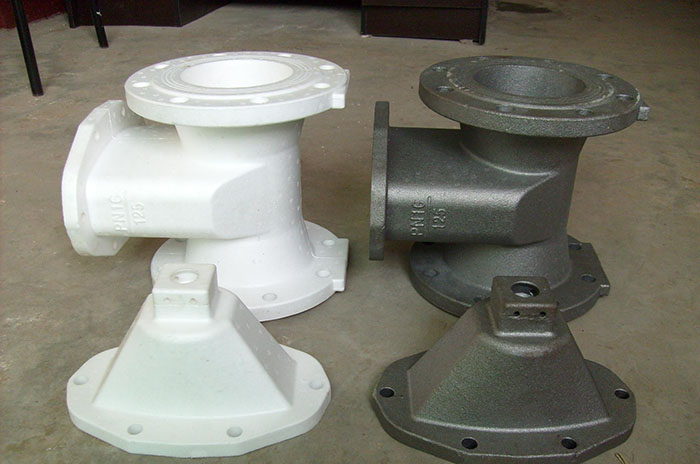
\includegraphics[width=4cm]{./R-C.jpg}
\end{center}
\end{column}
\end{columns}
\end{frame}

\begin{frame}[label={sec:orgf0e02be}]{壳型铸造}
\begin{itemize}
\item 使用细二氧化硅或锆石砂与热固性树脂粘合制备薄壳模具
\end{itemize}
\begin{columns}
\begin{column}{0.5\columnwidth}
\begin{center}
\includegraphics[page=295, viewport={70.0 413.5 282.5 656.5}, clip,width=6cm]{./WorkshopProcesses.pdf}
\end{center}
\end{column}
\begin{column}{0.5\columnwidth}
\begin{center}
\includegraphics[page=295, viewport={306.0 428.5 494.5 657.5}, clip,width=6cm]{./WorkshopProcesses.pdf}
\end{center}
\end{column}
\end{columns}
\end{frame}

\begin{frame}[label={sec:org02ec708}]{压铸}
\begin{itemize}
\item 高压(5 \(\sim\) 150MPa)、高速充型
\end{itemize}
\begin{center}
\includegraphics[page=51, viewport={259.5 62.9 547.0 278.4}, clip,width=8cm]{./metaljixiehot.pdf}
\end{center}
\end{frame}

\begin{frame}[label={sec:org3b233f3}]{常见铸造缺陷}
\begin{columns}
\begin{column}{0.25\columnwidth}
气孔
\begin{center}
\includegraphics[page=53, viewport={201.5 618.4 369.5 696.9}, clip,width=3cm]{./metaljixiehot.pdf}
\end{center}
\end{column}
\begin{column}{0.25\columnwidth}
缩孔
\begin{center}
\includegraphics[page=53, viewport={240.0 347.4 331.0 419.9}, clip,width=2cm]{./metaljixiehot.pdf}
\end{center}
\end{column}
\begin{column}{0.25\columnwidth}
砂眼
\begin{center}
\includegraphics[page=53, viewport={219.5 527.4 351.5 604.4}, clip,width=3cm]{./metaljixiehot.pdf}
\end{center}
\end{column}

\begin{column}{0.25\columnwidth}
渣眼
\begin{center}
\includegraphics[page=53, viewport={216.5 437.4 352.5 515.4}, clip,width=3cm]{./metaljixiehot.pdf}
\end{center}
\end{column}
\end{columns}
\begin{columns}
\begin{column}{0.25\columnwidth}
冷隔
\begin{center}
\includegraphics[page=53, viewport={197.0 65.4 372.0 150.4}, clip,width=3cm]{./metaljixiehot.pdf}
\end{center}
\end{column}
\begin{column}{0.25\columnwidth}
浇不足
\begin{center}
\includegraphics[page=54, viewport={239.0 639.4 317.5 717.9}, clip,width=2cm]{./metaljixiehot.pdf}
\end{center}
\end{column}
\begin{column}{0.25\columnwidth}
错箱
\begin{center}
\includegraphics[page=54, viewport={198.0 548.4 369.5 621.4}, clip,width=3cm]{./metaljixiehot.pdf}
\end{center}
\end{column}

\begin{column}{0.25\columnwidth}
裂纹
\begin{center}
\includegraphics[page=53, viewport={218.0 253.9 355.5 328.9}, clip,width=3cm]{./metaljixiehot.pdf}
\end{center}
\end{column}
\end{columns}
\end{frame}

\section{锻造}
\label{sec:org19637b8}

\begin{frame}[label={sec:orgf674109}]{锻造}
下料\(\rightarrow\) 加热 \(\rightarrow\) 锻造 \(\rightarrow\) 冷却 \(\rightarrow\) 热处理 \(\rightarrow\) 清理 \(\rightarrow\) 检验 \(\rightarrow\) 锻件

\begin{columns}
\begin{column}{0.6\columnwidth}
\begin{itemize}
\item 加热是为提高塑性，均匀化内部组织
\item \alert{始锻温度} ：允许加热的最高温度
\item \alert{终锻温度} ：金属停止锻造时的温度，需要重新加热才能继续锻造
\item \alert{过热} ：温度过高或高温停留时间过长，组织迅速长大变粗的现象，可用正火或调质进行消除
\item \alert{过烧} ：温度接近熔化温度，晶粒间结合力完全丧失，该缺陷无法消除
\end{itemize}
\end{column}
\begin{column}{0.4\columnwidth}
\begin{center}
\includegraphics[page=61, viewport={70.5 140.9 185.5 283.4}, clip,width=4cm]{./metaljixiehot.pdf}
\end{center}

1 下砧铁 2 锻件 3 上砧铁
\end{column}
\end{columns}
\end{frame}

\begin{frame}[label={sec:org3ea2497}]{常用金属材料的锻造温度范围}
\begin{itemize}
\item 不出现过热或过烧的前提下始锻温度 \alert{尽量高}
\item 保证停锻前金属有足够的塑性的前提下，终锻温度 \alert{尽量低}
\end{itemize}

\begin{center}
\includegraphics[page=64, viewport={48.5 507.9 553.0 676.4}, clip,width=11cm]{./metaljixiehot.pdf}
\end{center}
\end{frame}

\begin{frame}[label={sec:orgc050062}]{自由锻工具}
\begin{center}
\includegraphics[page=67, viewport={86.0 54.3 528.0 391.6}, clip,width=11cm]{./metaljixiehot.pdf}
\end{center}
\end{frame}

\begin{frame}[label={sec:org4f8d2b2}]{自由锻工序}
\begin{columns}
\begin{column}{0.5\columnwidth}
\begin{center}
\includegraphics[page=69, viewport={94.7 220.3 512.7 452.3}, clip,width=6cm]{./metaljixiehot.pdf}
\end{center}
\end{column}
\begin{column}{0.5\columnwidth}
\begin{center}
\includegraphics[page=73, viewport={134.0 587.6 466.7 762.3}, clip,width=6cm]{./metaljixiehot.pdf}
\end{center}
\end{column}
\end{columns}

\begin{columns}
\begin{column}{0.5\columnwidth}
\begin{center}
\includegraphics[page=72, viewport={296.0 118.3 544.0 322.9}, clip,width=6cm]{./metaljixiehot.pdf}
\end{center}
\end{column}
\begin{column}{0.5\columnwidth}
\begin{center}
\includegraphics[page=73, viewport={161.3 52.3 436.0 252.9}, clip,width=6cm]{./metaljixiehot.pdf}
\end{center}
\end{column}
\end{columns}
\end{frame}

\begin{frame}[label={sec:org7bca224}]{闭式模锻 Close-die forging}
\begin{itemize}
\item 将金属置于上下锻模的型槽中，上下模对击驱使金属流动，充满型槽得到锻件
\item \alert{单模膛锻模} ：仅有一个成形模膛
\item 多数情况通常需要一系列模具并经历多个道次（ \alert{多模膛锻模} ）
\item 每个道次逐渐改变形状，直到获得最终形状（\fKai 拔长模膛、滚压模膛、变曲模膛、预锻模膛、终锻模膛\normalfont ）
\end{itemize}
\begin{center}
\includegraphics[page=275, viewport={337.5 51.0 463.5 124.0}, clip,width=6cm]{./WorkshopProcesses.pdf}
\end{center}
\end{frame}

\begin{frame}[label={sec:orge47e9ff}]{自由锻和模锻视频}
\begin{columns}
\begin{column}{0.5\columnwidth}
\href{https://www.bilibili.com/video/BV1hW411u72k/?share_source=copy_web&vd_source=065b5817f3e3c58ce8d6353b4192b896}{B站拔长视频} \qrcode[height=2cm]{https://www.bilibili.com/video/BV1hW411u72k/?share_source=copy_web&vd_source=065b5817f3e3c58ce8d6353b4192b896}
\end{column}
\begin{column}{0.5\columnwidth}
\href{https://www.bilibili.com/video/BV11SbJ6rENs/?share_source=copy_web&vd_source=065b5817f3e3c58ce8d6353b4192b896}{手锤模锻} \qrcode[height=2cm]{https://www.bilibili.com/video/BV11SbJ6rENs/?share_source=copy_web&vd_source=065b5817f3e3c58ce8d6353b4192b896}
\end{column}
\end{columns}
\end{frame}

\begin{frame}[label={sec:org03e1894}]{锤上模锻与压力机上模锻}
\begin{itemize}
\item 锤上模锻依靠 \alert{冲击力} 成形，精度不高、振动和噪声大
\item 压力机（\fKai 液压及机械压力\normalfont ）上模锻振动小、易维护、操作简单
\end{itemize}

\begin{center}
\includegraphics[page=76, viewport={78.3 527.4 512.0 684.1}, clip,width=10cm]{./manufactextbook.pdf}
\end{center}
\end{frame}

\begin{frame}[label={sec:org97c1314}]{轧制 Rolling}
\begin{itemize}
\item 通过旋转轧辊对金属坯料施加压力，使其产生连续塑性变形，从而改变截面形状、尺寸和性能
\item 厚度减薄、长度增加、宽度略有增加，保持体积守恒
\item 热轧（\fKai 再结晶温度以上\normalfont ）、冷轧（\fKai 室温或再结晶温度以下\normalfont ）和温轧（\fKai 介于冷轧、热轧之间\normalfont ）
\end{itemize}
\begin{center}
\includegraphics[page=273, viewport={109.5 267.0 244.5 338.5}, clip,width=7cm]{./WorkshopProcesses.pdf}
\end{center}
\end{frame}

\begin{frame}[label={sec:org8cd6990}]{挤压 Extrusion}
\begin{itemize}
\item 生产任意复杂截面的产品
\item 表面质量好、尺寸精度高
\item 材料受挤压出，相对脆性材料也可挤压
\end{itemize}
\begin{columns}
\begin{column}{0.5\columnwidth}
\begin{figure}[htbp]
\centering
\includegraphics[page=274, viewport={36.0 232.0 230.5 360.5}, clip,width=6cm]{./WorkshopProcesses.pdf}
\caption{直接挤压}
\end{figure}
\end{column}
\begin{column}{0.5\columnwidth}
\begin{figure}[htbp]
\centering
\includegraphics[page=274, viewport={268.0 540.5 450.5 658.5}, clip,width=6cm]{./WorkshopProcesses.pdf}
\caption{间接挤压}
\end{figure}
\end{column}
\end{columns}
\end{frame}

\begin{frame}[label={sec:org8e89e06}]{拉拔 Drawing}
\begin{itemize}
\item 用于生产线材和棒材
\item 保持良好润滑，提高模具寿命和线材表面质量
\end{itemize}
\begin{center}
\includegraphics[page=275, viewport={70.5 265.5 283.0 356.5}, clip,width=10cm]{./WorkshopProcesses.pdf}
\end{center}
\end{frame}

\section{冲压加工}
\label{sec:org8dde1e7}

\begin{frame}[label={sec:org383aed7}]{冲压加工}
\begin{itemize}
\item 对金属板材施加力，使其发生变形（如弯曲）或分离（落料或冲孔）的过程
\item 凸模和凹模之间的间隙以每侧加工材料厚度的百分比表示（\fKai 参照标准或手册\normalfont ）
\begin{itemize}
\item 薄料、软料、精度高时间隙 \alert{取小值} ，厚料、硬料、提高模具寿命时 \alert{取大值}
\end{itemize}
\end{itemize}
\begin{columns}[b]
\begin{column}{0.5\columnwidth}
\begin{figure}[htbp]
\centering
\includegraphics[page=282, viewport={294.5 50.0 421.0 143.5}, clip,width=5cm]{./WorkshopProcesses.pdf}
\caption{凸模凹模的剪切作用}
\end{figure}
\end{column}
\begin{column}{0.5\columnwidth}
\begin{figure}[htbp]
\centering
\includegraphics[page=283, viewport={116.0 589.5 235.0 666.0}, clip,width=5cm]{./WorkshopProcesses.pdf}
\caption{剪切边的特点}
\end{figure}
\end{column}
\end{columns}
\end{frame}

\begin{frame}[label={sec:org225c20e}]{落料 Blanking}
\begin{itemize}
\item 用落料模从坯料上冲下所需的毛坯，冲剩的是余料
\end{itemize}

\begin{center}
\includegraphics[page=47, viewport={213.9 191.0 460.0 257.5}, clip,width=10cm]{./npupractice.pdf}
\end{center}
\end{frame}
\begin{frame}[label={sec:org3fa057f}]{排样}
\begin{itemize}
\item 冲压件坯件的形状和大小在板料或条料上排列布置的方式
\begin{itemize}
\item 有废料排样：坯料全部外形周边有搭边或余料
\item 少废料排样：局部周边有搭边或余料
\item 无废料排样：无任何搭边或余料
\end{itemize}
\end{itemize}

\begin{center}
\includegraphics[page=86, viewport={97.3 78.3 503.3 196.9}, clip,width=8cm]{./metaljixiehot.pdf}
\end{center}
\end{frame}
\begin{frame}[label={sec:orgb7c409d}]{冲孔 Piecing}
\begin{itemize}
\item 用冲孔模在板料或工件上冲出所需的孔，被冲下的是余料
\end{itemize}

\begin{center}
\includegraphics[page=47, viewport={225.2 115.4 470.9 184.1}, clip,width=10cm]{./npupractice.pdf}
\end{center}
\end{frame}

\begin{frame}[label={sec:orgb2fabd3}]{落料冲孔凸凹模尺寸计算}
\begin{itemize}
\item 凸模决定冲孔尺寸大小，凹模决定落料尺寸的大小
\item 冲孔时冲出的材料为废料，落料时冲出的材料的产品
\end{itemize}
\begin{center}
\includegraphics[page=283, viewport={328.5 548.5 454.0 665.5}, clip,width=6cm]{./WorkshopProcesses.pdf}
\end{center}
\end{frame}

\begin{frame}[label={sec:org00a787d}]{弯曲}
\begin{itemize}
\item 弯曲是变形工序，弯曲时坯料内层被压缩，易起皱；外层受拉伸，易拉裂
\item 弯曲线尽可能与板料纤维组织方向垂直
\item 弯曲半径越小，变形程度越大，各种材料均有规定的最小许可弯曲半径
\item 弯曲后会回弹一个角度，所以冲头角度略小于工件的角度
\end{itemize}
\begin{center}
\includegraphics[page=89, viewport={147.5 58.4 455.0 224.9}, clip,width=10cm]{./metaljixiehot.pdf}
\end{center}
\end{frame}

\begin{frame}[label={sec:orgd5ba1eb}]{拉深}
\begin{itemize}
\item 坯料（\fKai 通常由落料获得\normalfont）在冲模具作用下成为杯形或盒形工件
\item 冲头和凹模边缘做成圆角，避免拉深时开裂
\item 深度大的拉深件需多道次拉深而成
\item 拉深时金属发生加工硬化，还需进行退火处理，以恢复塑性
\end{itemize}

\begin{center}
\includegraphics[page=48, viewport={72.6 480.2 330.4 574.9}, clip,width=10cm]{./npupractice.pdf}
\end{center}
\end{frame}

\begin{frame}[label={sec:orge6486dc}]{变薄拉深 Ironing(取``熨烫''一义)}
\begin{itemize}
\item 凸模与凹模之间的间隙小于坯料的原始厚度
\item 经过初步拉深成形的空心杯状件（预成形件）被推过这个狭窄间隙时，侧壁金属在均匀压应力作用下发生塑性变形
\begin{itemize}
\item 壁厚变薄，高度增加，底部厚度保持不变
\end{itemize}
\item 适合制造高度大、壁薄而底厚的圆筒形零件
\begin{itemize}
\item 易拉罐、弹壳、高压容器、波纹管等
\end{itemize}
\end{itemize}

\href{https://www.bilibili.com/video/BV17zGiz1ELt}{巨型乙炔瓶制造} \qrcode[height=2cm]{https://www.bilibili.com/video/BV17zGiz1ELt/?share_source=copy_web&vd_source=065b5817f3e3c58ce8d6353b4192b896}
\end{frame}

\section{参考教材}
\label{sec:org4d810f2}
\begin{frame}[label={sec:orga904df0}]{参考教材}
\begin{enumerate}
\item 耿俊浩（译），机械制造基础及实践（Workshop Processes, Practices and Materials 5th Edition），北京：机械工业出版社，2023.9
\item 黄明宇，金属实习（下册，冷加工，第3版），北京：机械工业出版社，2025.2
\item 柳秉毅，金工实习（上册，热加工，第2版），北京：机械工业出版社，2009.4
\item 北航、西工大合编，金工实习，北京：国防工业出版社，
\end{enumerate}
\end{frame}
\end{document}
